%%%%%%%%%%%%%%%%%%%%%%%%%%%%%%%%%%%%%%%%%%%%%%%%
% Boissier Florian
% Ducoroy  Laurent
% Voronin  Marc
% L3 Info
%%%%%%%%%%%%%%%%%%%%%%%%%%%%%%%%%%%%%%%%%%%%%%%%
\documentclass[french]{report}
\usepackage[T1]{fontenc}
\usepackage[utf8]{inputenc}
\usepackage{lmodern}
\usepackage[a4paper]{geometry}
\usepackage{graphicx} % Images
\usepackage{titlepic} % Logo première page
\usepackage{mathtools} % Maths
\usepackage{amssymb} % Maths
\usepackage{esvect} % Vecteurs de meilleurs qualité
\usepackage{array} % Tableaux
\usepackage{siunitx} % Unités internationnales
\usepackage{babel} % Accents
\usepackage[pageanchor=false]{hyperref} % Liens, etc.
% Les liens amènent correctement aux images et non aux légendes
\usepackage[all]{hypcap} 

% Macros
\DeclarePairedDelimiter\abs{\lvert}{\rvert}% % Valeur absolue

\tcbset{fonttitle=\bfseries,separator sign none, description delimiters parenthesis}
\newtcbtheorem{dem}{Démonstration}{colback=green!5!white,colframe=green!75!black}{}

% Vecteur 3d affiché en colonne
% Param #1: le nom du vecteur
% Param #2-4: x, y et z
\newcommand{\vvv}[4]{%
	\vv{#1}\left(
		\begin{tabular}{c}
			#2 \\ #3 \\ #4 \\
		\end{tabular}
	\right)
}

% cos alpha/2
\newcommand{\cosad}{	
	\cos \frac{\alpha}{2}
}

% sin alpha/2
\newcommand{\sinad}{	
	\sin \frac{\alpha}{2}
}

% cos² alpha/2
\newcommand{\coscad}{	
	\cos^2 \frac{\alpha}{2}
}

% sin² alpha/2
\newcommand{\sincad}{	
	\sin^2 \frac{\alpha}{2}
}

% cos alpha
\newcommand{\cosa}{\cos \alpha}

% sin alpha
\newcommand{\sina}{\sin \alpha}

% v ^ u
\newcommand{\vecsc}[2]{
	\vec{#1} \wedge \vec{#2}
}

% v . u
\newcommand{\vecpr}[2]{
	\vec{#1} \cdot \vec{#2}
}

% 1 / 4
\newcommand{\qter}{
	\frac{1}{4}
}

% Ecriture simplifiées
\newcommand{\Q}[2]{
	Q_{#1#2}
}

\newcommand{\Qxx}{
	\Q{x}{x}
}

\newcommand{\Qxy}{
	\Q{x}{y}
}

\newcommand{\Qxz}{
	\Q{x}{z}
}

\newcommand{\Qyx}{
	\Q{y}{x}
}

\newcommand{\Qyy}{
	\Q{y}{y}
}

\newcommand{\Qyz}{
	\Q{y}{z}
}

\newcommand{\Qzx}{
	\Q{z}{x}
}

\newcommand{\Qzy}{
	\Q{z}{y}
}

\newcommand{\Qzz}{
	\Q{z}{z}
}

% Matrice 1 colonne et 4 lignes
\newcommand{\moq}[4]{
	\left(
		\begin{tabular}{c}
			$#1$ \\
			$#2$ \\
			$#3$ \\
			$#4$
		\end{tabular}
	\right)
}

% Première page
\title{Rapport Unité D'ouverture: \LaTeX}
\author{Boissier Florian\thanks{boissierflorian@outlook.com} \and Ducoroy Laurent\thanks{l.ducoroy@gmail.com} \and Voronin Marc\thanks{voronin.mark123@gmail.com}}
\titlepic{
\includegraphics[width=5cm]{ressources/logo_ulco}}

\begin{document}

\maketitle
\tableofcontents
\listoffigures
	
% Fichiers principal (A ré-organiser si nécessaire)
\begin{abstract}
\begin{center}
		Rapport, d'une dizaine de pages et en \LaTeX, sur le \lang\cplus.
\end{center}
\end{abstract}
\chapter{Introduction}
\section{Qu'est-ce que le C++ ?}
Vous vous demandez sûrement par où commencer, si le \cplus est fait pour vous, s'il n'est pas préférable de démarrer avec un autre \lang. Vous vous demandez si vous allez pouvoir faire tout ce que vous voulez, quelles sont les forces et les faiblesses du \cplus…

Dans ce chapitre, je vais tenter de répondre à toutes ces questions. 
N'oubliez pas : \emph{c'est un cours pour débutants. Aucune connaissance préalable n'est requise.} 
\section{Les \progs}
Les \progs sont à la base de l'informatique. Ce sont eux qui vous permettent d'exécuter des actions sur votre \ordi.

Prenons par exemple la \fig \ref{troisfen} qui représente une capture d'écran de mon \ordi. On y distingue \nb{3} fenêtres correspondant à \nb{3} \progs différents.
Du premier plan à l'arrière plan :

\fimg{./images/trois_fenetres}{Trois fenêtres}{troisfen}
\begin{itemize}
	\item le navigateur web \textbf{Google Chrome}, qui permet de consulter des sites web;
	\item l'explorateur de fichiers, qui permet de gérer les fichiers de son \ordi;
	\item le traitement de texte \textbf{Microsoft Word}, qui permet de rédiger lettres et documents. 
\end{itemize}

Comme vous le voyez, chacun de ces \progs est conçu dans un but précis. On pourrait aussi citer les jeux, par exemple, qui sont prévus pour s'amuser : \textbf{Starcraft \nb{2}} (\fig \ref{scdeux}), \textbf{World of Warcraft},\textbf{ Worms}, \textbf{Team Fortress \nb{2} } , etc. Chacun d'eux correspond à un \prog différent.

\fimg{ducoroy/images/starcraft}{Starcraft II}{scdeux}




\emph{Tous les \progs ne sont pas forcément visibles. C'est le cas de ceux qui surveillent les mises à jour disponibles pour votre \ordi ou, dans une moindre mesure, de votre antivirus. Ils tournent tous en \guill{tâche de fond}, ils n'affichent pas toujours une fenêtre ; mais cela ne les empêche pas d'être actifs et de travailler !}

Votre \ordi est une machine étonnante et complexe. À la base, il ne comprend qu'un \lang très simple constitué de \nb{0} et de \nb{1}. 
Pour se simplifier la vie, les informaticiens ont créé des \langs intermédiaires, plus simples que le binaire.

 Il existe aujourd'hui des centaines de \langs de \progio. Pour vous faire une idée, vous pouvez consulter une liste des \langs de \progio sur \textbf{Wikipédia}. Chacun de ces \langs a des spécificités, nous y reviendrons.
Tous les \langs de \progio ont le même but : vous permettre de parler à l'\ordi plus simplement qu'en binaire. Voici comment cela fonctionne :

\begin{enumerate}
	\item Vous écrivez des instructions pour l'\ordi dans un \lang de \progio (par exemple le \cplus) ;
	\item Les instructions sont traduites en binaire grâce à un \prog de \guill{traduction} ;
	\item L'\ordi peut alors lire le binaire et faire ce que vous avez demandé !
\end{enumerate}

Résumons ces étapes dans un schéma (\fig \ref{compil}).
\fimg{ducoroy/images/compilation}{Compilation}{compil}
\fimg{ducoroy/images/compilation_details}{La compilation en détails}{compildetail}

Le fameux \guill{\prog de traduction} s'appelle en réalité le \emph{compilateur}. C'est un outil indispensable. Il vous permet de transformer votre code, écrit dans un \lang de \progio, en un vrai \prog exécutable.

Reprenons le schéma précédent et utilisons un vrai vocabulaire d'informaticien (figure \ref{compildetail}).
Voilà ce que je vous demande de retenir pour le moment : ce n'est pas bien compliqué mais c'est la base à connaître absolument !


\section{Le C++ face aux autres \langs}
\subsection{Le C++ : \lang de haut niveau ou de bas niveau ?}
Parmi les centaines de \langs de \progio qui existent, certains sont plus populaires que d'autres. Sans aucun doute, le \cplus est un \lang \emph{très populaire}.

La question est : faut-il choisir un \lang parce qu'il est populaire ? Il existe des \langs très intéressants mais peu utilisés. Le souci avec les \langs peu utilisés, c'est qu'il est difficile de trouver des gens pour vous aider et vous conseiller quand vous avez un problème. Voilà entre autres pourquoi le \cplus est un bon choix pour qui veut débuter : il y a suffisamment de gens qui développent en \cplus pour que vous n'ayez pas à craindre de vous retrouver tous seuls !

C'est un \lang assez éloigné du binaire (et donc du fonctionnement de la machine), qui vous permet généralement de développer de façon plus souple et rapide.
Par opposition, un \lang de bas niveau est plus proche du fonctionnement de la machine : il demande en général un peu plus d'efforts mais vous donne aussi plus de contrôle sur ce que vous faites. C'est à double tranchant.

Le \cplus ? On considère qu'il fait partie de la seconde catégorie : c'est un \lang dit  de \guill{bas niveau}. Mais que cela ne vous fasse pas peur ! Même si le \cplus peut se révéler assez complexe, vous aurez entre les mains un \lang très puissant et particulièrement rapide. En effet, si l'immense majorité des jeux sont développés en \cplus, c'est parce qu'il s'agit du \lang qui allie le mieux puissance et rapidité. Voilà ce qui en fait un \lang incontournable.

Le schéma suivant représente quelques \langs de \progio classés par  \guill{niveau} (\fig \ref{langbyniv}).
\fimg{ducoroy/images/niveaux_langages}{Langages par niveau}{langbyniv}

Vous constaterez qu'il est en fait possible de \progrer en binaire grâce à un \lang très basique appelé l'assembleur.

\subsection{Petit aperçu du C++}
Pour vous donner une idée, voici un \prog très simple affichant le message \guill{Hello world!} à l'écran. Ce sera l'un des premiers codes source que nous étudierons dans les prochains chapitres.
\listinfo{C++}{listings/codes/premier_code.cpp}






\subsection{Résumé des forces du C++}
\begin{itemize}
	\item Il est très répandu. Comme nous l'avons vu, il fait partie des \langs de \progio les plus utilisés sur la planète. On trouve donc beaucoup de documentation sur Internet et on peut facilement avoir de l'aide sur les forums. 
	\item Il est rapide, très rapide même, ce qui en fait un \lang de choix pour les applications critiques qui ont besoin de performances. C'est en particulier le cas des jeux vidéo, mais aussi des outils financiers ou de certains \progs militaires qui doivent fonctionner en temps réel.
	\item Il est portable : un même code source peut théoriquement être transformé sans problème en exécutable sous \textbf{Windows}, \textbf{Mac OS} et \textbf{Linux}. 
	\item Il existe de nombreuses bibliothèques pour le \cplus. Les bibliothèques sont des extensions pour le \lang, un peu comme des plug-ins. De base, le \cplus ne sait pas faire grand chose mais, en le combinant avec de bonnes bibliothèques, on peut créer des \progs 3D, réseaux, audio, fenêtrés, etc.
	\item Il est multi-paradigmes. Ce mot barbare signifie qu'on peut \progrer de différentes façons en \cplus. Vous êtes encore un peu trop débutants pour que je vous présente tout de suite ces techniques de \progio mais l'une des plus célèbres est la \emph{Programmation Orientée Objet (POO)}. C'est une technique qui permet de simplifier l'organisation du code dans nos \progs et de rendre facilement certains morceaux de codes réutilisables. 
	
\end{itemize}
\chapter{Votre premier \prog}
\section{Le monde merveilleux de la console}
Quand je vous annonce que nous allons commencer à \progrer, vous vous dites sûrement\textit{ « Chouette, je vais pouvoir faire ça, ça et ça ; et j'ai toujours rêvé de faire ça aussi ! »}. Il est de mon devoir de calmer un peu vos ardeurs et de vous expliquer comment cela va se passer.

Nous allons commencer doucement. Nous n'avons de toute façon pas le choix car les \progs complexes 3D en réseau que vous imaginez peut-être nécessitent de connaître les bases.

Il faut savoir qu'il existe 2 types de \progs : les \progs graphiques et les \progs console.
\subsection{Les \progs graphiques}
Il s'agit des \progs qui affichent des fenêtres. Ce sont ceux que vous connaissez sûrement le mieux. Ils génèrent à l'écran des fenêtres que l'on peut ouvrir, réduire, fermer, agrandir…
Les programmeurs parlent de \emph{GUI} (Graphical User Interface - Interface Utilisateur Graphique voir \fig \ref{gui}). 
\fimg{ducoroy/images/gui}{Un programme \textsc{gui} (graphique)}{gui}

\subsection{Les \progs console}
Les \progs en console sont plus fréquents sous \textbf{Linux} que sous \textbf{Windows} et \textbf{Mac OS X}. Ils sont constitués de simples textes qui s'affichent à l'écran, le plus souvent en blanc sur fond noir (\fig \ref{console}).

\fimg{ducoroy/images/console}{Un programme en console)}{console}
Ces \progs fonctionnent au clavier. La souris n'est pas utilisée.
Ils s'exécutent généralement linéairement : les messages s'affichent au fur et à mesure, de haut en bas.
\subsection{Notre première cible : les \progs console}
Je vous annonce que nous allons commencer par réaliser des \progs console. En effet, bien qu'ils soient un peu austères \textit{à priori}, ces \progs sont beaucoup plus simples à créer que les \progs graphiques.
\section{Explications sur ce premier code source}
Lorsque \textbf{Code::Blocks} crée un nouveau projet, il génère un fichier \lstinline|main.cpp| contenant ce code :

\listinfo{C++}{listings/codes/premier_code.cpp}






\subsection{include}
La toute première ligne est : \partlist{C++}{1-1}{./listings/codes/premier_code.cpp}
C'est ce qu'on appelle une \emph{directive de préprocesseur}. Son rôle est de \guill{charger} des fonctionnalités du \cplus pour que nous puissions effectuer certaines actions.

En effet, \emph{le \cplus est un \lang très modulaire}. De base, il ne sait pas faire grand-chose (pas même afficher un message à l'écran !). On doit donc charger des extensions que l'on appelle bibliothèques et qui nous offrent de nouvelles possibilités.

Ici on charge le fichier \lstinline!iostream!, ce qui nous permet d'utiliser une bibliothèque… d'affichage de messages à l'écran dans une console !

\subsection{using namespace}
\partlist{C++}{2-2}{./listings/codes/premier_code.cpp}
… permet en quelque sorte d'indiquer dans quel lot de fonctionnalités notre fichier source va aller piocher.

Si vous chargez plusieurs bibliothèques, chacune va proposer de nombreuses fonctionnalités. Parfois, certaines fonctionnalités ont le même nom. Imaginez une commande \guill{AfficherMessage} qui s'appellerait ainsi pour \lstinline|iostream| mais aussi pour \lstinline|Qt| ! Si vous chargez les deux bibliothèques en même temps et que vous appelez \guill{AfficherMessage}, l'\ordi ne saura pas s'il doit afficher un message en console avec \lstinline|iostream| ou dans une fenêtre avec \lstinline|Qt| !

Pour éviter ce genre de problèmes, on a créé des \emph{namespaces} (espaces de noms), qui sont des sortes de dossiers à noms. La ligne \lstinline|using namespace std;| indique que vous allez utiliser l'espace de noms \lstinline|std| dans la suite de votre fichier de code. Cet espace de noms est un des plus connus car il correspond à la bibliothèque standard (\lstinline|std|), une bibliothèque livrée par défaut avec le \lang \cplus et dont \lstinline|iostream| fait partie.

\subsection{int main}
C'est ici que commence vraiment le cœur du \prog. Les \progs, vous le verrez, sont essentiellement constitués de fonctions. Chaque fonction a un rôle et peut appeler d'autres fonctions pour effectuer certaines actions.
Tous les \progs possèdent une fonction dénommée \guill{main} (Qui se prononce \guill{mèïne} en anglais.), ce qui signifie \guill{principale}. C'est donc la fonction principale.

Une fonction à la forme suivante :

\listinfo{C++}{listings/codes/codevide.cpp}
Au bout de la fonction \lstinline|main| le \prog s'arrête ! Tout \prog commence au début de la fonction \lstinline|main| et se termine à la fin de celle-ci.

\subsection{cout}
Voici enfin la première ligne qui fait quelque chose de concret ! C'est la première ligne de \lstinline|main|, donc la première action qui sera exécutée par l'\ordi (les lignes que nous avons vues précédemment ne sont en fait que des préparatifs pour le \prog).

\partlist{C++}{5-5}{./listings/codes/premier_code.cpp}
Le rôle de \lstinline|cout| (à prononcer \guill{ci aoute}) est d'afficher un message à l'écran. C'est ce qu'on appelle une instruction. Tous nos \progs seront constitués d'instructions comme celle-ci, qui donnent des ordres à l'\ordi.

Notez que \lstinline|cout| est fourni par \lstinline|iostream|. Si vous n'incluez pas \lstinline|iostream| au début de votre \prog, le compilateur se plaindra de ne pas connaître \lstinline|cout| et vous ne pourrez pas générer votre \prog !

\subsection{return}
La dernière ligne est :
\partlist{C++}{6-6}{./listings/codes/premier_code.cpp}

Ce type d'instruction clôt généralement les fonctions. En fait, la plupart des fonctions renvoient une valeur (un nombre par exemple). Ici, la fonction \lstinline|main| renvoie \nb{0} pour indiquer que tout s'est bien passé (toute valeur différente de \nb{0} aurait indiqué un problème).

Vous n'avez pas besoin de modifier cette ligne, laissez-la telle quelle. Nous aurons d'autres occasions d'utiliser \lstinline|return| pour d'autres fonctions, nous en reparlerons !

\section{Commentez et mettez en forme vos \progs !}
En plus du code qui donne des instructions à l'\ordi, vous pouvez écrire des commentaires pour expliquer le fonctionnement de votre \prog.

Les commentaires n'ont aucun impact sur le fonctionnement de votre logiciel : en fait, le compilateur ne les lit même pas et ils n'apparaissent pas dans le \prog généré. Pourtant, ces commentaires sont indispensables pour les développeurs : ils leur permettent d'expliquer ce qu'ils font dans leur code !

\subsection{Différents types de commentaires}
Il y a deux façons d'écrire des commentaires selon leur longueur. Je vais vous les présenter toutes les deux.

\subsubsection{Commentaires courts}
Pour écrire un commentaire court, sur une seule ligne, il suffit de commencer par \lstinline|//| puis d'écrire votre commentaire. Cela donne :

\partlist{C++}{1-1}{./listings/codes/commentaires.cpp}

Mieux, vous pouvez aussi ajouter le commentaire à la fin d'une ligne de code pour expliquer ce qu'elle fait :

\partlist{C++}{2-2}{./listings/codes/commentaires.cpp}

\subsubsection{Commentaires longs}

\partlist{C++}{3-6}{./listings/codes/commentaires.cpp}


\chapter{Utiliser la mémoire}
\section{Introduction}
Jusqu'à présent, vous avez découvert comment créer et compiler vos premiers \progs en mode console. Pour l'instant ces \progs sont très simples. Ils affichent des messages à l'écran… et c'est à peu près tout.
Mais avant cela, il va nous falloir travailler dur puisque je vais vous présenter une notion fondamentale en informatique. Nous allons parler des\emph{ \varis}.
\section{Qu'est-ce qu'une \vari ?}
La seule et unique chose que vous ayez besoin de savoir, c'est qu'une \vari est une partie de la mémoire que l'\ordi nous prête pour y mettre des valeurs. Imaginez que l'\ordi possède dans ses entrailles une grande armoire (\fig \ref{tiroirs}). Cette dernière possède des milliers (des milliards !) de petits tiroirs ; ce sont des endroits que nous allons pouvoir utiliser pour mettre nos \varis.

\fimg{./images/tiroirs}{La mémoire d'un ordinateur fonctionne comme une grosse armoire avec beaucoup de tiroirs}{tiroirs}
\subsection{Les noms de \varis}
Commençons par la question du nom des \varis. En \cplus, il y a quelques règles qui régissent les différents noms autorisés ou interdits :

\begin{itemize}
	\item les noms de \varis sont constitués de lettres, de chiffres et du tiret-bas \_ uniquement;
	\item le premier caractère doit être une lettre (majuscule ou minuscule) ;
	\item on ne peut pas utiliser d'accents ;
	\item on ne peut pas utiliser d'espaces dans le nom.
\end{itemize}

 Le \lang fait la différence entre les majuscules et les minuscules. En termes techniques, on dit que \cplus est \emph{sensible à la casse}. Donc, \lstinline|nomZero|,  \lstinline|nomzero|,  \lstinline|NOMZERO| et \lstinline|NomZeRo| sont tous des noms de \varis différents.
\subsection{Les types de \varis}
Reprenons. Nous avons appris qu'une \vari a un nom et un type. Nous savons comment nommer nos \varis, voyons maintenant leurs différents types. L'\ordi aime savoir ce qu'il a dans sa mémoire, il faut donc indiquer quel type d'élément va contenir la \vari que nous aimerions utiliser. Est-ce un nombre, un mot, une lettre ? Il faut le spécifier.

Voici donc la liste des types de \varis que l'on peut utiliser en C++.


\begin{tabular}{cc}
	$Type$ & $Contenu$ \\
	\toprule
	bool & Une valeur parmi deux possibles, vrai (true) ou faux (false). \\
	\midrule
	char & Un caractère. \\
	\midrule
	int & Un nombre entier. \\
	\midrule
	unsigned int & Un nombre entier positif ou nul. \\
	\midrule
	double & Un nombre à virgule. \\
	\midrule
	string & Une chaîne de caractères, c'est-à-dire un mot ou une phrase. \\
	\bottomrule
\end{tabular}

\newtheorem{ bornes}{Note}
\begin{ bornes}
	Ces types ont des limites de validité, des bornes, c'est-à-dire qu'il y a des nombres qui sont trop grands pour un \lstinline|int| par exemple. Ces bornes dépendent de votre \ordi, de votre système d'exploitation et de votre compilateur. Sachez simplement que ces limites sont bien assez grandes pour la plupart des utilisations courantes. 
	Cela ne devrait donc pas vous poser de problème, à moins que vous ne vouliez créer des \progs pour téléphones portables ou pour des micro-contrôleurs, qui ont parfois des bornes plus basses que les \ordis.
	Il existe également d'autres types avec d'autres limites mais ils sont utilisés plus rarement.
\end{ bornes}



\chapter{Un peu de mathématiques}
\section{L'en-tête \lstinline|cmath|}
Pour avoir accès à plus de fonctions mathématiques, il suffit d'ajouter une ligne en tête de votre \prog, comme lorsque l'on désire utiliser des \varis de type \lstinline|string|. La directive à insérer est :

\partlist{C++}{2-2}{ducoroy/listings/codes/maths.cpp}

Commençons avec une fonction utilisée très souvent, la racine carrée. En anglais, racine carrée se dit \textit{square root} et, en abrégé, on écrit parfois \lstinline|sqrt|. Comme le \cplus utilise l'anglais, c'est ce mot là qu'il va falloir retenir et utiliser.

Pour utiliser une fonction mathématique, on écrit le nom de la fonction suivi, entre parenthèses, de la valeur à calculer. On utilise alors l'affectation pour stocker le résultat dans une \vari.

C'est comme en math quand on écrit $y = f(x)$. Il faut juste se souvenir du nom compliqué des fonctions. Pour la racine carrée, cela donnerait : \partlist{C++}{8-8}{ducoroy/listings/codes/maths.cpp}

Prenons un exemple complet, je pense que vous allez comprendre rapidement le principe.

\listinfo{C++}{listings/codes/maths.cpp}

\subsection{Le cas de la fonction puissance}
Comme toujours, il y a un cas particulier : la fonction puissance. Comment calculer $4^5?$

Si je veux calculer $4^5$, je vais devoir procéder ainsi :

\listinfo{C++}{ducoroy/listings/codes/calcul_puissance.cpp}     
%%%%%%%%%%%%%%%%%%%%%%%%%%%%%%%%%%%%%%%%%%%%%%%%
% Boissier Florian
% Fichier personel principal: boissier/rapport.tex
% L3 Info
%%%%%%%%%%%%%%%%%%%%%%%%%%%%%%%%%%%%%%%%%%%%%%%%

\chapter{Quaternions et rotation dans l'espace}
Les quaternions unitaires fournissent une notation mathématique commode pour représenter l'orientation et la rotation d'objets en trois dimensions. Comparés aux angles d'Euler, ils sont plus simple à composer et évitent le problème du blocage de cardan. Comparés aux matrices de rotations, ils sont plus stables numériquement et peuvent se révéler plus efficaces. Les quaternions ont été adoptés dans des applications en infographie, robotique, navigation, dynamique moléculaire et la mécanique spatiale des satellites.

\section{Opérations de rotation à l'aide de quaternions}
Une explication très stricte des propriétés utilisées dans cette section est donnée par Altmann\label{Altmann}.

	\subsection{L'hypersphère des rotations}
		\subsubsection{Se faire une idée de l'espace des rotations}
			Les quaternions unitaires représentent l'\emph{espace mathématique} des rotations en trois dimensions de façon relativement simple. On peut comprendre la correspondance entre les rotations et les quaternions en commençant d'abord par se faire une idée intuitive de l'espace des rotations lui-même.
Deux rotations d'angles différents et d'axes différents dans l'espace des rotations. La norme du vecteur est liée à l'amplitude de la rotation.

Chaque rotation en trois dimensions consiste à tourner d'un certain angle autour d'un certain axe. Quand l'angle est nul, l'axe n'a pas d'importance, de telle façon qu'une rotation de zéro degré est un simple point dans l'espace des rotations (c'est la rotation identité). Pour un angle petit mais non nul, l'ensemble des rotations possibles est une petite sphère entourant la rotation identité, où chaque point de la sphère représente un axe pointant dans une direction particulière (comparez avec la sphère céleste). Des rotations d'angles de plus en plus grands s'éloignent progressivement de la rotation identité, et nous pouvons nous les représenter comme des sphères concentriques de rayons croissants. Par conséquent, au voisinage de la rotation identité, l'espace abstrait des rotations ressemble à l'espace ordinaire en trois dimensions (qui peut également être vu comme un point central entouré de sphères de différents rayons. La ressemblance s'arrête là : lorsque l'angle de rotation dépasse \ang{180}, les rotations suivant les différents axes cessent de diverger et commencent à nouveau à se ressembler, pour finir par devenir identiques (et égales à la rotation identité) lorsque l'angle atteint \ang{360}.

\begin{figure}[ht]
	\centering
	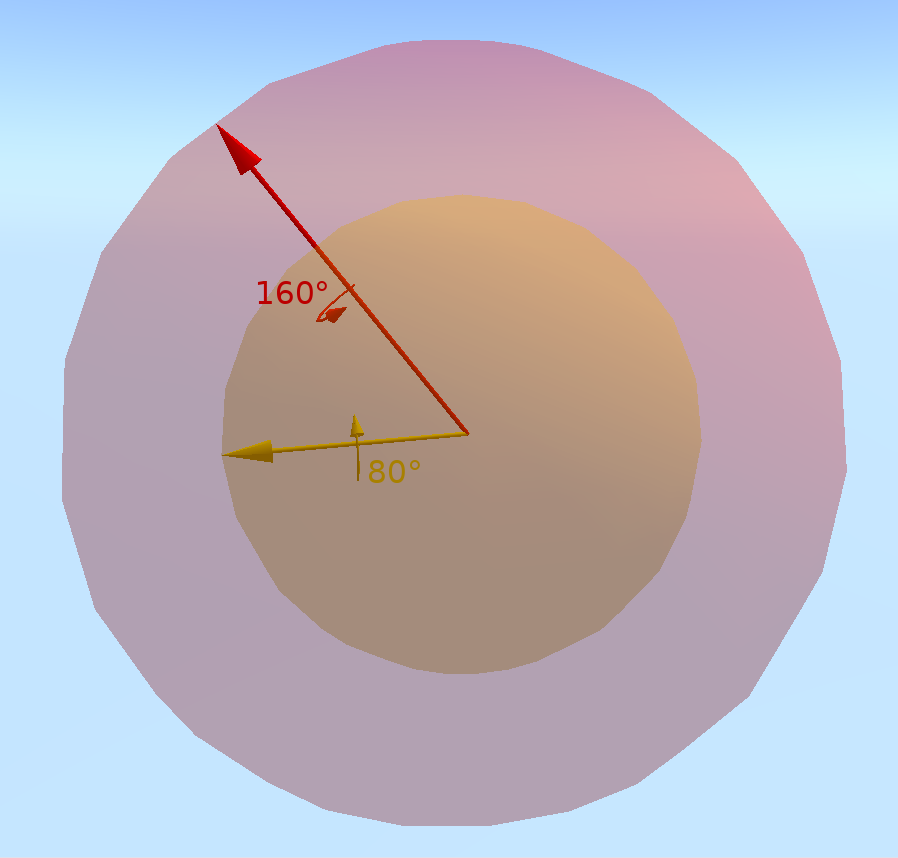
\includegraphics[width=5cm]{ressources/espace_rotations}\hfill
	\caption{Deux rotations d'angles différents et d'axes différents dans l'espace des rotations. La norme du vecteur est liée à l'amplitude de la rotation.}
	\label{espace_rotations}
\end{figure}

L'hypersphère des rotations pour les rotations d'axes horizontaux (axes compris dans le plan xy).
On constate un phénomène analogue à la surface d'une sphère. Si nous nous plaçons au pôle Nord et traçons à partir de là des lignes droites (en fait, des méridiens) dans plusieurs directions, elles divergeront puis convergeront à nouveau au pôle Sud. Des cercles concentriques de rayon croissant dessinés autour du pôle Nord (des parallèles) finiront par s'effondrer en un point au pôle Sud une fois que l'on a parcouru la distance entre les pôles. On peut assimiler les différentes directions à partir du pôle (c'est-à-dire les différents méridiens) aux différents axes de rotations et les différentes distances au pôle Nord aux différents angles : on a ainsi une analogie de l'espace des rotations. Mais la surface de la sphère est en deux dimensions alors que les \emph{axes} de rotation utilisent déjà trois dimensions. L'espace des rotations est donc modélisé par une sphère de dimension 3 dans un espace à 4 dimensions (une hypersphère). Nous pouvons penser à la sphère ordinaire comme à une section de l'hypersphère, de la même façon qu'un cercle est une section de sphère. On peut prendre la section pour représenter, par exemple, uniquement les rotations d'axes dans le plan $xy$ (voir illustration ci-contre). On remarque que l'angle de la rotation est deux fois la différence de latitude avec le pôle Nord : en effet, les points de l'équateur représentent des rotations de \ang{180}, pas de \ang{90}, et le pôle Sud représente la rotation identité de \ang{360}, et pas le demi-tour de \ang{180}.

Le pôle Nord et le pôle Sud représentent la même rotation, et en fait cela s'applique à n'importe quelle paire de points aux antipodes l'un de l'autre : si un point correspond à une rotation d'angle $\alpha$ autour de l'axe dirigé par le vecteur $\vv{v}$, l'autre point correspond à une rotation d'angle $\text{\ang{360}} - \alpha$ autour de l'axe dirigé par le vecteur $\vv{v}$. En fait, l'espace des rotations n'est pas l'hypersphère elle-même, mais l'hypersphère où l'on identifie les points aux antipodes l'un de l'autre. Mais dans un but de simplification, nous pouvons penser aux rotations comme à des points de la sphère en dimension 4, même si la moitié de ces points est redondante (revêtement double).

\begin{figure}[ht]
	\centering
	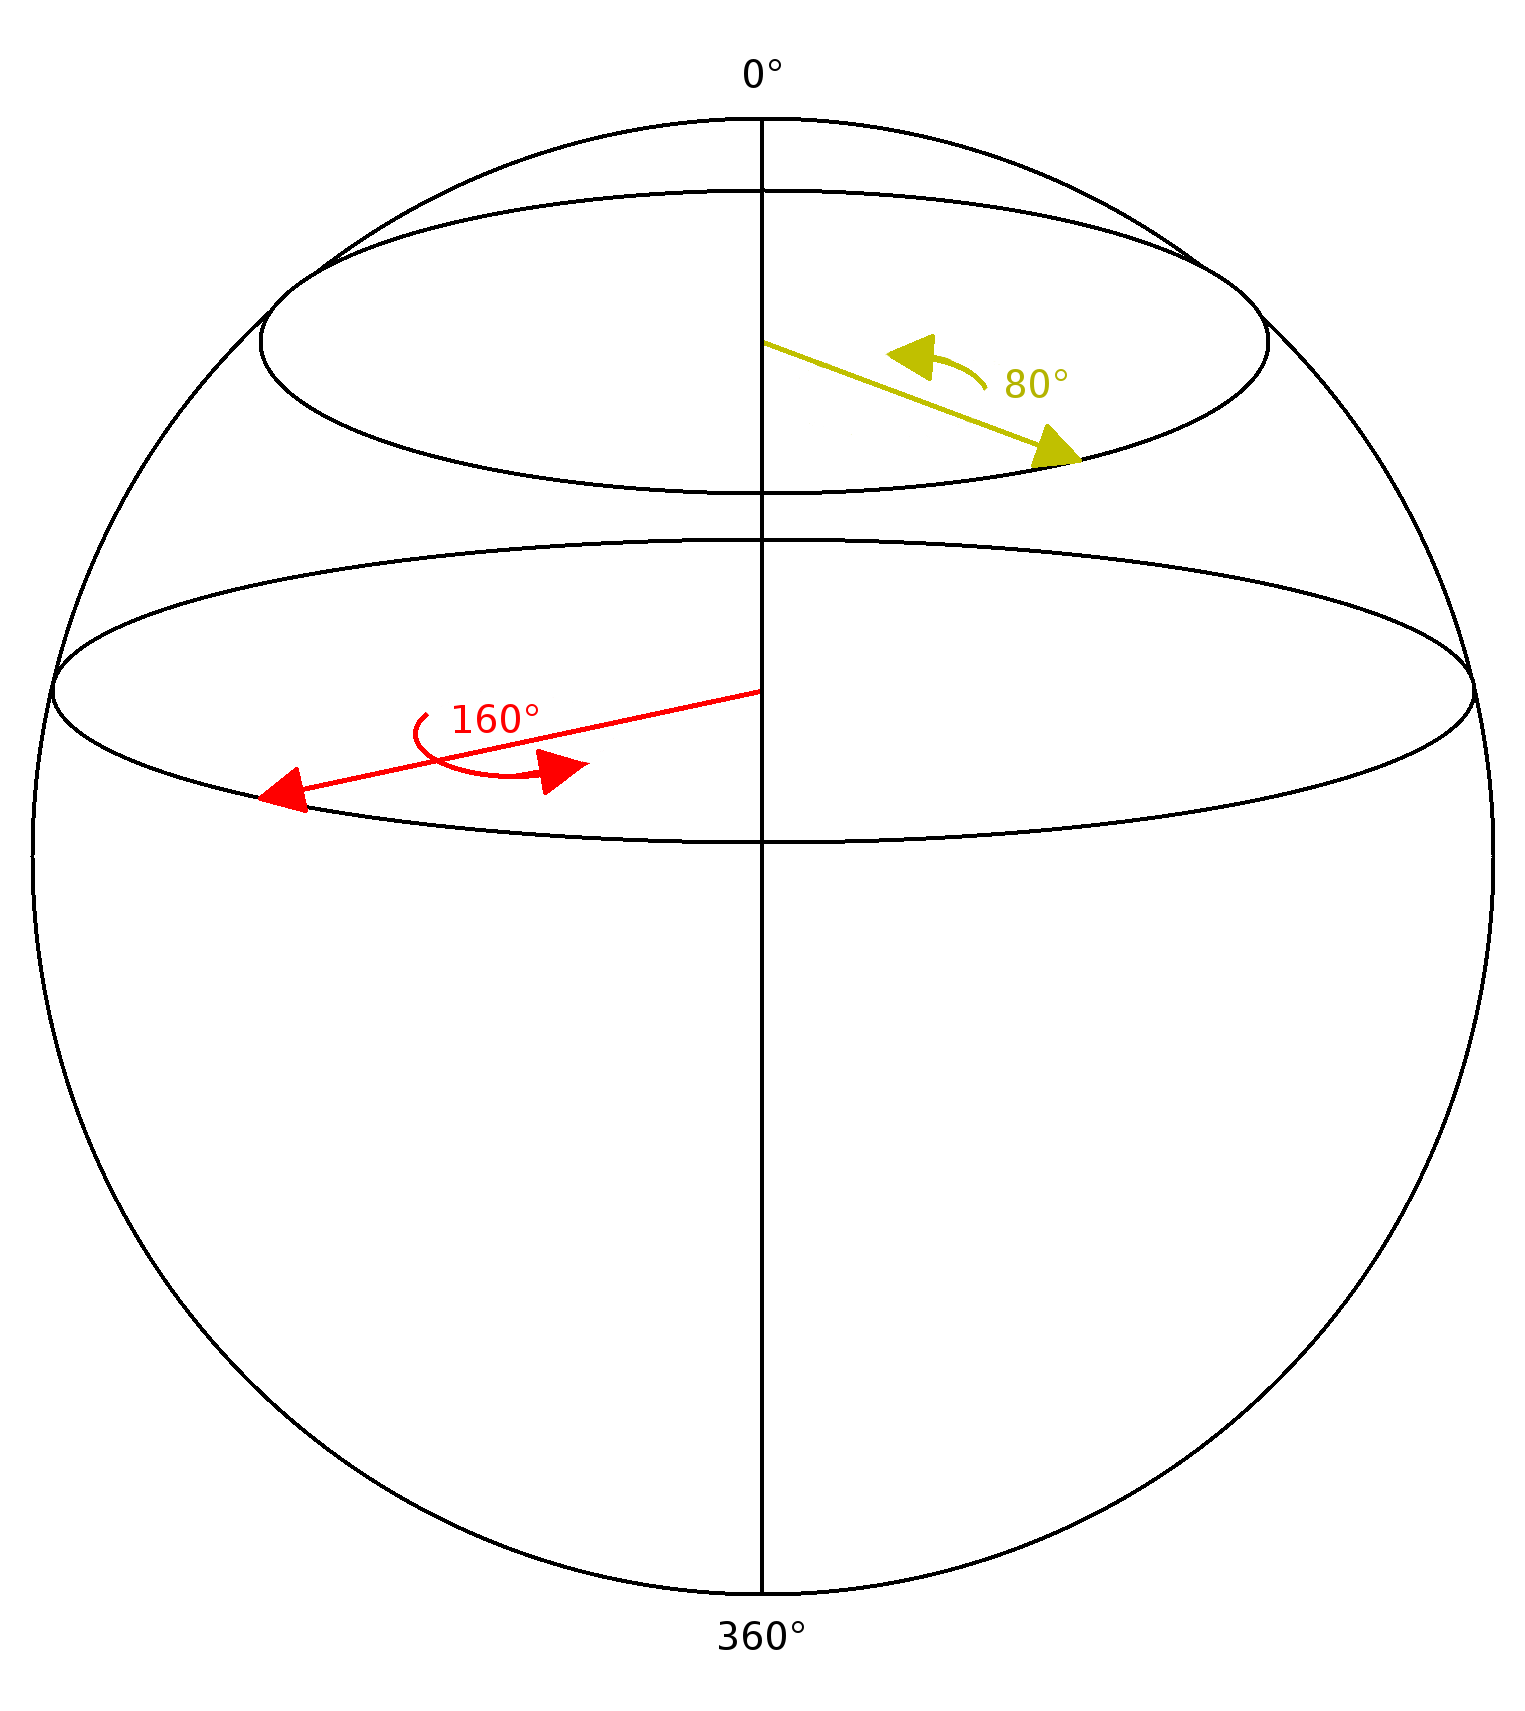
\includegraphics[width=5cm,height=4cm]{ressources/hypersphere_rotations}\hfill
	\caption{L'hypersphère des rotations pour les rotations d'axes horizontaux (axes compris dans le plan $xy$).}
	\label{hypersphere_rotations}
\end{figure}
		\subsubsection{Paramétrer l'espace des rotations}
			Nous pouvons paramétrer la surface d'une sphère à l'aide de deux coordonnées, comme la latitude et la longitude. 
Mais la latitude et la longitude se comportent mal (sont dégénérés) aux pôles Nord et Sud, 
alors que les pôles ne sont pas différents par nature des autres points de la sphère. 
Aux pôles Nord et Sud (de latitudes $+$\ang{90} et $-$\ang{90}), la longitude perd son sens.

On peut montrer qu'aucun système de coordonnées à deux paramètres ne peut éviter cette dégénérescence 
(c'est le théorème de la boule chevelue). Nous pouvons éviter de tels problèmes en plongeant la sphère 
dans l'espace à trois dimensions et en la paramétrant au moyen de trois coordonnées 
cartésiennes (ici $w$, $x$ et $y$), en plaçant le pôle Nord à $(w, x, y) = (1, 0, 0)$, 
le pôle Sud à $(w, x, y) = ( -1, 0, 0)$ et l'équateur sera le cercle d'équations 
$w = 0 \text{et} x^2 + y^2 = 1$. Les points de la sphère satisfont la contrainte $w^2 + x^2 + y^2 = 1$, 
donc nous avons toujours deux degrés de liberté, bien que l'on ait trois coordonnées. 
Un point $(w, x, y)$ de la sphère représente une rotation de l'espace ordinaire autour 
de l'axe horizontal dirigé par le vecteur $\vvv{v}{x}{y}{0}$ et d'angle 
$\alpha = 2\cos^{-1} w = 2 \sin^{-1}\sqrt{x^2+y^2}$.

De la même façon, l'hypersphère décrivant l'espace des rotations dans l'espace en trois dimensions 
peut être paramétrée au moyen de trois angles (angles d'Euler), mais tout paramétrage de ce type 
dégénère en certains points de l'hypersphère, ce qui conduit au problème du blocage de cardan. 
Nous pouvons éviter cela en utilisant quatre coordonnées euclidennes $w, x, y et z$, 
avec $w^2 + x^2 + y^2 + z^2 = 1$. Le point de coordonnées $(w, x, y, z)$ représente une rotation 
autour de l'axe dirigé par le vecteur $\vvv{v}{x}{y}{z}$
et d'angle $\alpha = 2\cos^{-1} w = 2 \sin^{-1}\sqrt{x^2+y^2+z^2}$.
	\subsection{Des rotations aux quaternions}
		\subsubsection{Les quaternions en bref}
			On peut définir les nombres complexes en introduisant un symbole abstrait $i$ qui se conforme aux 
règles usuelles de l'algèbre et qui en plus obéit à la règle $i^2 = - 1$. 
Cela suffit à reproduire toutes les règles de calcul des nombres complexes, 
par exemple: 
\[
(a + bi)(c + di) = ac + adi + bic + bidi = ac + adi + bci + bdi^{2} = (ac - bd) + (bc + ad) i
\]

De la même façon, les quaternions peuvent être définis en introduisant des symboles abstraits 
$i, j \text{et} k$ qui satisfont aux règles $i^2 = j^2 = k^2 = ijk = -1$ et les règles 
algébriques usuelles \emph{sauf} la commutativité de la multiplication (un exemple familier 
de multiplication non commutative est la multiplication des matrices). L'ensemble des règles 
de calcul découle de ces définitions ; par exemple, on peut montrer que 
\begin{align*}
(a+bi+cj+dk)(e+fi+gj+hk) &= (ae-bf-cg-dh)+(af+be+ch-dg)i+ \\
(ag+ce+df-bh)j + (ah+de+bg-cf)k.
\end{align*}

La partie imaginaire $bi+cj+dk$ d'un quaternion se comporte comme un vecteur $\vvv{v}{b}{c}{d}$
 d'un espace vectoriel à trois dimensions et la partie réelle $a$ comme un scalaire de $\mathbb{R}$.

Quand les quaternions sont utilisés en géométrie, il est pratique de les définir comme un 
scalaire plus un vecteur: $a+bi+cj+dk = a + \vec{v}$

Ceux qui ont étudié les vecteurs à un niveau élémentaire pourraient trouver étrange d'additionner 
un \emph{nombre} à un vecteur, car ce sont des objets de natures très différentes, ou de 
\emph{multiplier} deux vecteurs entre eux, car cette opération n'est d'habitude pas définie.
 Néanmoins, si l'on se souvient qu'il ne s'agit là que d'une notation pour les parties réelles et 
 imaginaires d'un quaternion, cela devient plus légitime.

Nous pouvons exprimer la multiplication de quaternions (produit de Hamilton) dans le langage moderne 
du produit vectoriel et du produit scalaire de vecteurs (qui ont en fait été inspirés au début par 
les quaternions). À la place des règles $i^2=j^2=k^2=ijk=-1$, nous avons la règle de multiplication 
de deux vecteurs $\vec{v}\vec{w}=\vec{v}\wedge\vec{w}-\vec{v}\cdot\vec{w}$, où:

\begin{itemize}
	\item $\vec{v}\vec{w}$ est la multiplication de vecteurs,
	\item $\vec{v}\wedge\vec{w}$ est le produit vectoriel (un vecteur),
	\item $\vec{v}\cdot\vec{w}$ est le produit scalaire un nombre).s
\end{itemize}

La multiplication de vecteurs n'est pas commutative (à cause du produit vectoriel), alors que la 
multiplication entre scalaires et entre un scalaire et un vecteur sont commutatives. Il découle de
 manière immédiate de ces règles que $(s + \vec{v})(t + \vec{w}) = (st - \vec{v}\cdot\vec{w}) + 
 (s\vec{w}+t\vec{v}+\vec{v}\wedge\vec{w})$.

L'inverse (à gauche et à droite) d'un quaternion non nul est $(s + \vec{v})^-1 = 
\frac{s - \vec{v}}{s^2 + \abs{\vec{v}}^2}$, comme cela peut être vérifié par calcul direct.
		\subsubsection{Relation entre les rotations et les quaternions unitaires}
			Soient $(w, x, y, z)$ les coordonnées d'une rotation, comme décrit précédemment. 
Définissons le quaternion : $q = w + xi + yj+ zk = w + \vvv{v}{x}{y}{z} = 
\cos( \alpha / 2 ) + \vec{u} \sin( \alpha/2 )$
où $\vec{u}$ est un vecteur unitaire. Soit également $\vec{v}$ un vecteur
ordinaire de l'espace en 3 dimensions, considéré comme un quaternion avec
une coordonnée réelle nulle. On peut alors montrer (voir section suivante) 
que le produit de quaternions: 
\[
q\vec{v}q^-1
\]
renvoie le vecteur $\vec{v}$ tourné d'un angle $\alpha$ autour de l'axe dirigé
par $\vec{u}$.La rotation se fait dans le sens des aiguilles d'une montre 
si notre ligne de vue pointe dans la même direction que $\vec{u}$.Cette opération 
est connue comme la conjugaison par $q$.

Il s'ensuit que la multiplication de quaternions correspond à la composition de 
rotations, car si $p \text{et} q$ sont des quaternions représentant des rotations, 
alors la rotation (conjugaison) par $pq$ est:
\[
pq\vec{v}( pq )^-1 = pq\vec{v}q^-1p^-1 = p( q\vec{v}q^-1 )p^-1 \text{,}
\]
ce qui revient à tourner (conjuguer) par $q$, puis par $p$.

Le quaternion inverse d'une rotation correspond à la rotation inverse, car
$q^-1( q\vec{v}q^-1 )q = \vec{v}$.

Le carré d'un quaternion correspond à la 
rotation de deux fois le même angle autour du même axe. Plus généralement, 
$q^n$ correspond à une rotation de $n$ fois l'angle autour du même axe que $q$.
Cela peut être étendu à un réel arbitraire n, ce qui permet de calculer des rotations intermédiaires de façon fluide entre des rotations de l'espace, c'est
\emph{l'interpolation linéaire sphérique}.
		\subsubsection{Démonstration de l'équivalence entre conjugaison de quaternions et rotation de l'espace}
			Soit $\vec{u}$ un vecteur unitaire (l'axe de rotation) et soit 
$q = \cos \frac{\alpha}{2} + \vec{u} \sin \frac{\alpha}{2}$.

Notre but est de montrer que :

\[
	\vv{v'} = q\vec{v}q^-1 = ( \cos \frac{\alpha}{2} + 
	\vec{u} \sin \frac{\alpha}{2} ) \vv{v} ( \cos 
	\frac{\alpha}{2} - \vv{u} \sin \frac{\alpha}{2} )
\]

renvoie le vecteur $\vec{v}$ tourné d'un angle $\alpha$ autour de l'axe
dirigé par $\vec{u}$.

En développant, on obtient en effet :

\begin{align*}
	\vv{v'} & = \vv{v} \coscad + (\vec{u} \vec{v} - \vec{v}\vec{u}) \sinad \cosad- \vec{u}\vec{v}\vec{u}\sincad \\
	& = \vv{v}\coscad + 2 ( \vecsc{u}{v}) \sinad \cosad - (\vec{v}(\vec{u} 
	\cdot \vec{u})) \sincad \\
	& = \vec{v}( \coscad - \sincad ) + (\vecsc{u}{v}) (2 \sinad \cosad) + \vv{u}(\vecpr{u}{v}) (2
	\sincad) \\ 
	& = \vec{v} \cosa + (\vecsc{u}{v}) \sina + \vec{u}(\vecpr{u}{v})( 1 - \cosa ) \\
	& = (\vec{v} - \vec{u}(\vecpr{u}{v})) \cosa + (\vecsc{u}{v}) \sina + \vec{u}(\vecpr{u}{v}) \\
	& = \vec{v}_{\perp} \cosa + (\vecsc{u}{v}_{\perp}) \sina + \vec{v}_{\|}
\end{align*}

où $\vec{v}_{\perp} \text{ et } \vec{v}_{\|}$ sont les composantes de $\vec{v}$ 
respectivement orthogonale et colinéaire à $\vec{u}$. C'est là la formule de 
\bsc{Olinde Rodrigues} qui donne la rotation d'angle $\alpha$ autour de l'axe dirigé par $\vec{u}$.
	\subsection{Exemple}
	
\section{Expliquer les propriétés des quaternions à l'aide des rotations}
	\subsection{Non-commutativité}
	\subsection{Les quaternions sont-ils orientés ?}
	
\section{Les quaternions et les autres représentations des rotations}
	\subsection{Description qualitative des avantages des quaternions}
	\subsection{Conversion vers et depuis la représentation sous forme de matrice}
		\subsubsection{D'un quaternion en matrice orthogonale}
		\subsubsection{D'une matrice orthogonale en quaternion}
		\subsubsection{Quaternions optimaux}
	\subsection{Comparaisons de performances avec d'autres méthodes de rotation}
		\subsubsection{Résultats}
		\subsubsection{Méthodes utilisées}
\section{Les paires de quaternions unitaires comme rotations dans l'espace à 4 dimensions}

\chapter{Débuter avec HTML/CSS}
Ce court tutoriel est destiné à  ceux qui commencent à  utiliser CSS et n'ont jamais écrit de feuille de style CSS.

Il n'explique pas CSS en profondeur. Il explique comment créer un fichier HTML, un fichier CSS et comment les faire fonctionner ensemble. Après cela, vous pourrez lire d'autres tutoriels afin d'ajouter plus de caractéristiques à  vos fichiers HTML et CSS. Ou bien vous pouvez utiliser un éditeur HTML ou CSS afin de mettre en place des sites complexes.

A la fin de ce tutoriel, vous aurez fait un fichier HTML qui ressemble à cela (voir figure \ref{fig:screen1}). 

\begin{figure}[h]
	\begin{center}
		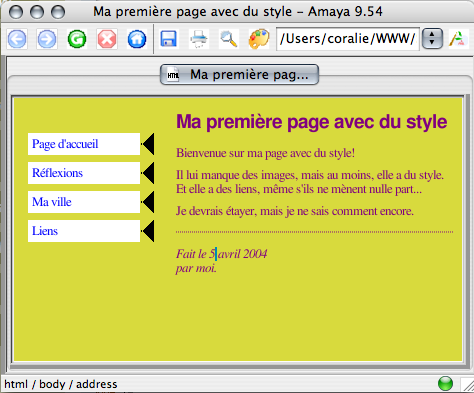
\includegraphics{voronin/img/capture5.png}	
		\caption{Page HTML résultante, couleurs et disposition effectuées avec CSS.}
		\label{fig:screen1}
	\end{center}
\end{figure}
Notez que je ne prétends pas que c'est joli :)
\alerte{3}{l}
Voici un exemple de section \emph{optionnelle}. Elles contiennent des explications supplémentaires du langage HTML et TML et du code CSS des exemples. L'icône "alerte!" qui les précède indique que la section contient des informations plus avancées que le reste.
\normalsize
\section{Le langage HTML}
Pour ce tutoriel, je vous recommande d'utiliser des outils simples comme Blocnote (Windows), TextEdit (Mac) ou KEdit (KDE). Une fois que vous aurez intégré ces principes, vous pourrez facilement utiliser des outils plus avancés, ou des logiciels commerciaux tels que Style Master, Dreamweaver ou GoLive. Cependant pour votre première feuille de style CSS, il vaut mieux que vous ne soyez pas distrait par de nombreuses caractéristiques avancées.

N'utilisez pas un logiciel de traitement de texte, tels que Microsoft Word ou OpenOffice, car ils produisent des fichiers qu'un navigateur Web ne sait pas lire. Pour HTML et CSS, nous voulons de simples fichiers texte.

\textbf{L'étape 1} est d'ouvrir votre éditeur de texte (Notepad, TextEdit, KEdit, etc., quel que soit votre éditeur favori), de commencer avec une fenêtre vide et de taper ceci:
\begin{lstlisting}[language=html]
	<!DOCTYPE html PUBLIC "-//W3C//DTD HTML 4.01//EN">
	<html>
	<head>
	<title>Ma premiere page avec du style</title>
	</head>
	
	<body>
	
	<!-- Menu de navigation du site -->
	<ul class="navbar">
	<li><a href="index.html">Home page</a>
	<li><a href="reflexions.html">Reflexions</a>
	<li><a href="ville.html">Ma ville</a>
	<li><a href="liens.html">Liens</a>
	</ul>
	
	<!-- Contenu principal -->
	<h1>Ma premiere page avec du style</h1>
	
	<p>Bienvenue sur ma page avec du style! 
	
	<p>Il lui manque des images, mais au moins, elle a du style. Et elle a des liens, meme s'ils ne menent nulle part...
	&hellip;
	
	<p>Je devrais etayer, mais je ne sais comment encore.
	
	<!-- Signer et dater la page, c'est une question de politesse! -->
	<address>Fait le 5 avril 2004<br>
	par moi.</address>
	</body>
	</html>
\end{lstlisting}
En fait, vous n'avez pas à le taper: vous pouvez le copier et coller depuis cette page Web dans votre éditeur.

(Si vous utilisez TextEdit sur Mac, n'oubliez pas de dire à TextEdit qu'il s'agit de texte simple; pour ceci, allez au menu Format et sélectionnez "Convertir au format Texte".) 
\alerte{13}{l}
 La première ligne du fichier HTML ci-dessus dit au navigateur de quel type d'HTML il s'agit (DOCTYPE signifie DOCument TYPE). Dans ce cas, il s'agit de la version 4.01 d'HTML.
 
 Les mots à l'intérieur de < et > sont nommés balises et comme vous pouvez le voir, le document est contenu à l'intérieur des balises <html> et </html>. Entre <head> et </head> se trouve la place pour des informations variées qui ne sont pas affichées à l'écran. A ce stade, il contient le titre du document, mais plus tard, nous y ajouterons la feuille de style CSS.
 
 Le <body> est l'emplacement du texte à proprement parler de notre document. En principe, tout ce qui s'y trouve sera affiché, à l'exception du texte contenu entre entre <!-- et -->, qui sert de commentaire pour nous-même. Le navigateur ignorera ce texte.
 
 Parmi les balises de l'exemple, <ul> introduit une "Liste non ordonnée", c'est à dire une liste dans laquelle les éléments ne sont pas numérotés. La balise <li> est le début d'un "élément de liste ". Le <p> est un "paragraphe". Et le <a> est une "ancre", ce qui crée un hyperlien(voir figure \ref{fig:screen2}). 

\begin{figure}[t]
	\begin{center}
		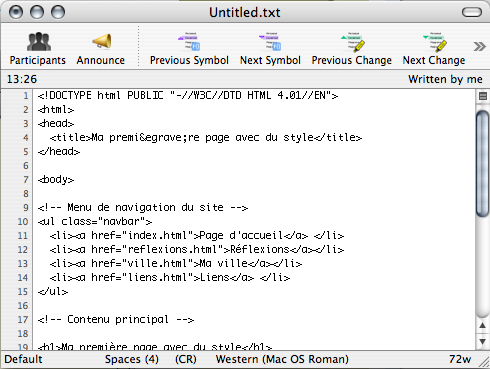
\includegraphics{voronin/img/capture.png}
		\caption{L'éditeur Subethaedit affichant le code source HTML.}
		\label{fig:screen2}		
	\end{center}
\end{figure}
\alerte{11}{l}
Si vous désirez connaître la signification du contenu d'un <…>, je vous recommande de commencer avec Getting started with HTML. Mais permettez-moi de vous livrer quelques mots sur la structure de la page HTML en exemple.
\begin{itemize}
	\item Le "ul" est une liste avec un hyperlien par élément. Cela nous servira de "menu de navigation de site," nous créerons des liens vers les autres pages de notre (hypothétique) site Web. Nous présumons que toutes les pages sur notre site ont un menu similaire.
	\item Les éléments "h1" et "p" forment le contenu unique de cette page, et la signature en bas ("address") sera similaire sur toutes les pages du site. 
\end{itemize}
Notez que je n'ai pas fermé les éléments "li" et "p". En langage HTML (mais pas en XHTML), il est permis d'omettre les balises </li> et </p>, ce que j'ai fait là, afin de rendre le texte un peu plus facile à lire. Mais vous pouvez les ajouter, si vous préférez. 
\normalsize

Admettons qu'il s'agira d'une page d'un site Web contenant plusieurs pages similaires. Comme dans beaucoup de pages Web actuelles, celle-ci a un menu avec des liens vers d'autres pages de notre site hypothétique, un contenu unique ainsi qu'une signature.

Sélectionnez maintenant "Sauver-sous…" depuis votre menu Fichier, naviguez vers le répertoire/dossier où vous voulez sauver votre fichier (le Bureau est tout à fait convenable) et sauvez le fichier sous le nom "mapage.html". Ne fermez pas l'éditeur car nous en aurons encore besoin.

(Si vous utilisez TextEdit sur Mac OS X avant version 10.4, vous voyez une option pour ne pas ajouter l'extension .txt. Sélectionnez cette option, parce que "mapage.html" a déjà une extension. Les versions plus récentes de TextEdit remarquent l'extension .html automatiquement.)

Ensuite, ouvrez le fichier dans un navigateur. Vous pouvez faire cela comme suit: cherchez le fichier avec votre explorateur de fichiers (Explorateur Windows, Finder ou Konqueror) et cliquez ou double-cliquez sur le fichier "mapage.html". Il devrait s'ouvrir dans votre navigateur Web par défaut. (Si ce n'est pas le cas, ouvrez votre navigateur et cliquez-déplacez le fichier dans le navigateur.)

Comme vous pouvez le voir, la page est assez ennuyeuse… 
\section{Ajouter de la couleur}
Vous voyez probablement du texte noir sur un fond blanc, mais cela dépend de la façon dont le navigateur est configuré. Une manière simple de rendre la page plus stylée et d'y ajouter des couleurs. (Laissez votre navigateur ouvert, nous l'utiliserons à nouveau plus tard.)

Nous allons commencer avec une feuille de style intégrée dans le fichier HTML. Par la suite, nous nous mettrons le HTML et le CSS dans des fichiers séparés. Séparer les fichiers est une bonne chose car cela vous permet facilement d'utiliser la même feuille de style sur plusieurs fichiers HTML: il vous suffit d'écrire votre feuille de style une fois. Mais pour cette cette étape, nous écrirons tout dans notre seul fichier.

Nous devons ajouter un élément <style> au fichier HTML. La feuille de style sera dans cet élément. Retournez à la fenêtre de votre éditeur et ajoutez les cinq lignes suivantes dans la partie head de votre fichier HTML. Les lignes à ajouter sont affichées en rouge. 
\begin{lstlisting}[language=html]
	<!DOCTYPE html PUBLIC "-//W3C//DTD HTML 4.01//EN">
	<html>
	<head>
	<title>Ma premiere page avec du style</title>
	<style type="text/css">
	body {
		color: purple;
		background-color: #d8da3d }
	</style>
	</head>
	
	<body>
	[etc.]
\end{lstlisting}
La première ligne indique qu'il s'agit d'une feuille de style et qu'elle est écrite en CSS ("text/css"). La seconde ligne indique que nous ajoutons du style à l'élément "body". La troisième ligne indique que la couleur du texte sera le violet, et la ligne suivante que le fond aura comme couleur une sorte de jaune verdâtre. 
\alerte{12}{l}
Les feuilles de style en CSS sont constituées de règles. Chacune des règles est en trois partie:
\begin{enumerate}
	\item Le sélecteur (dans l'exemple: "body"), qui indique au navigateur quelle partie du document est affectée par la règle;
	\item La propriété (dans l'exemple, 'color' et 'background-color' sont des propriétés), qui spécifie quel aspect de l'affichage est paramétré
	\item Et la valeur ('purple' et '\#d8da3d'), qui indique la valeur de la propriété de style. 
\end{enumerate}
L'exemple montre que les règles peuvent être combinées. Nous avons paramétré deux propriétés, donc nous aurions pu en faire deux règles séparées:

\begin{lstlisting}[language=html]
	body { color: purple }
	body { background-color: #d8da3d }
\end{lstlisting}

Mais puisque les deux règles affectent le corps ("body"), nous avons indiqué "body" une seule fois et mis les propriétés et valeurs ensemble. Pour en savoir plus sur les sélecteurs, se reporter au chapitre 2 de Lie \& Bos. 
\normalsize

Le fond de l'élément "body" sera également le fond de tout le document. Nous n'avons pas donné aux autres éléments (p, li, address…) de valeur explicite sur le fond, donc par défaut, ils n'en auront pas (ou plutôt: ils seront transparents). La propriété 'color' détermine la couleur du texte de l'élément "body", mais tous les autres éléments dans le corps hériteront de cette couleur, à moins qu'une autre soit spécifiée (Nous ajouterons d'autres couleurs plus plus tard.)

Sauvez maintenant ce fichier (utilisez "Sauver" depuis le menu Fichier) et retournez à la fenêtre de votre navigateur. Si vous pressez l'icône "Recharger", l'affichage devrait changer de la page "ennuyeuse" à une page colorée (mais certes toujours ennuyeuse) A part la liste de liens en haut, le texte devrait maintenant être violet sur un fond jaune verdâtre (voir figure \ref{fig:screen3}). 
\begin{figure}[t]
	\begin{center}
		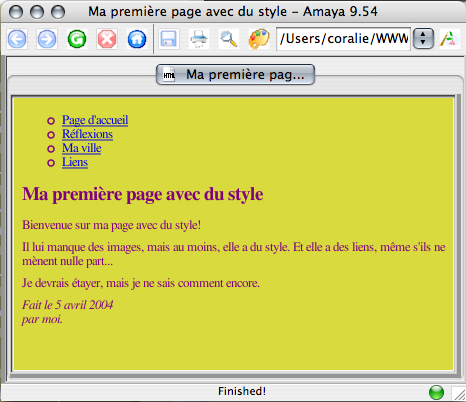
\includegraphics{voronin/img/capture2.png}	
		\caption{Voici comment un navigateur affiche la page maintenant que des couleurs ont été ajoutées. }
		\label{fig:screen3}
	\end{center}
\end{figure}
\alerte{6}{l}
En CSS, les couleurs peuvent être spécifiées de plusieurs manières. Cet exemple en montre deux: par nom ("purple") et par code hexadécimal ("\#d8da3d"). Il y a à peu prés 140 noms de couleurs. Les codes hexadécimaux permettent plus de 16 millions de couleurs. Adding a touch of style fournit plus d'explications à propos de ces codes. 
\normalsize
\section{Ajouter des fontes}
Une autre chose simple à faire est de distinguer les fontes des différents éléments de la page. Choisissons la fonte "Georgia", sauf pour le texte des titres de type h1 pour lesquels nous choisirons la fonte "Helvetica."

Sur le Web, vous ne pouvez jamais être sûr des fontes qu'auront vos lecteurs sur leurs ordinateurs, donc nous ajouterons des alternatives: si Georgia n'est pas disponible, Times New Roman ou Times iront très bien, et si ces deux-la sont également indisponibles, le navigateur pourra utiliser une autre fonte dans la famille serifs. Si Helvetica est absente, Geneva, Arial et SunSans-Regular sont assez similaire en forme, et si aucune de celles-ci ne fonctionne, le navigateur pourra choisir une autre fonte sans serif.

Dans votre éditeur de texte, ajoutez les lignes suivantes : 
\begin{lstlisting}[language=html]
	<!DOCTYPE html PUBLIC "-//W3C//DTD HTML 4.01//EN">
	<html>
	<head>
	<title>Ma premiere page avec du style</title>
	<style type="text/css">
	body {
		font-family: Georgia, "Times New Roman",
		Times, serif;
		color: purple;
		background-color: #d8da3d }
	h1 {
		font-family: Helvetica, Geneva, Arial,
		SunSans-Regular, sans-serif }
	</style>
	</head>
	
	<body>
	[etc.]
\end{lstlisting}
Si vous sauvez à nouveau et pressez "Recharger" dans le navigateur, vous devriez voir des fontes différentes pour le titre et le reste du texte (voir figure \ref{fig:screen4}).
\begin{figure}[t]
	\begin{center}
		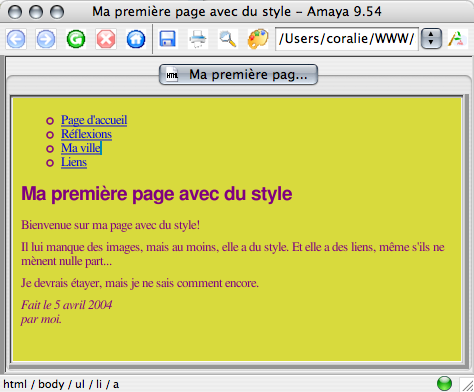
\includegraphics{voronin/img/capture3.png}	
		\caption{Maintenant le texte principal a une fonte différente de celle du titre.  }
		\label{fig:screen4}
	\end{center}
\end{figure} 
\section{La barre de navigation}
La liste en haut de la page HTML est sensée devenir un menu de navigation. Beaucoup de sites Web ont une sorte de menu en haut ou sur le côté de la page, et notre page devrait en avoir un aussi. Nous le mettrons du côté gauche, parce que c'est un peu plus intéressant qu'en haut…

Le menu est déjà dans la page HTML. Il s'agit de la liste <ul> en haut. Les liens à l'intérieur ne fonctionnent pas, puisque notre notre "site Web" consiste en une seule page, jusqu'à présent, donc ceci importe peu. Dans un site Web réel, il ne devrait pas y avoir de lien cassé, évidemment.

Nous devons donc déplacer la liste à gauche, et le reste du texte un petit peu à droite, pour faire de la place pour notre menu. Les propriétés CSS que nous utiliserons pour cela sont 'padding-left' (pour déplacer le texte du corps) et 'position', 'left' et 'top' (pour déplacer le menu).

Il y a d'autres manières de le faire. Si vous recherchez "column" ou "layout" dans la page Learning CSS, vous trouverez plusieurs modèles prêt à l'emploi. Mais cette manière convient à nos besoins.

Dans la fenêtre d'édition, ajoutez les lignes suivantes au fichier HTML : 
\begin{lstlisting}[language=html]
	<!DOCTYPE html PUBLIC "-//W3C//DTD HTML 4.01//EN">
	<html>
	<head>
	<title>Ma premiere page avec du style</title>
	<style type="text/css">
	body {
		padding-left: 11em;
		font-family: Georgia, "Times New Roman",
		Times, serif;
		color: purple;
		background-color: #d8da3d }
	ul.navbar {
		position: absolute;
		top: 2em;
		left: 1em;
		width: 9em }
	h1 {
		font-family: Helvetica, Geneva, Arial,
		SunSans-Regular, sans-serif }
	</style>
	</head>
	
	<body>
	[etc.]
\end{lstlisting}

Si vous sauvez encore et rechargez la page dans votre navigateur, vous devriez maintenant avoir la liste de liens à gauche du texte principal. C'est déjà bien plus intéressant, n'est-ce pas? (voir figure \ref{fig:screen5})
\begin{figure}[t]
	\begin{center}
		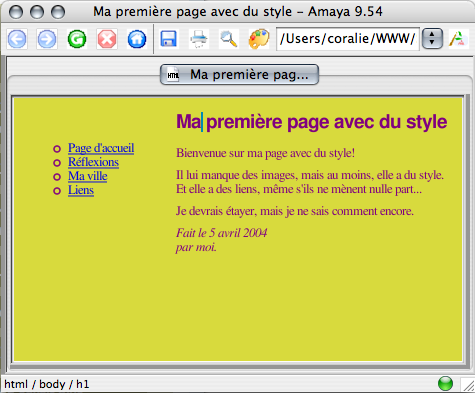
\includegraphics{voronin/img/capture4.png}	
		\caption{Le texte principal a été déplacé à droite et la liste de liens est maintenant à sa gauche au lieu d'être au-dessus. }
		\label{fig:screen5}
	\end{center}
\end{figure}
\alerte{12}{l}
'position: absolute' précise que l'élément ul est positionné de façon indépendante de tout texte qui vient avant ou après dans le document, et 'left' et 'top' indiquent quelle est cette position. Dans ce cas, 2em depuis le haut et 1em depuis le côté gauche de cette fenêtre.

'2em' signifie 2 fois la taille de la fonte courante. C'est à dire que si le menu est affiché avec une fonte de 12 points, '2em' font 24 points. L'unité 'em' est très utile en CSS puisqu'elle peut s'adapter automatiquement à la fonte que le lecteur utilise. La plupart des navigateurs ont un menu pour agrandir et réduire la taille de fonte: vous pouvez l'essayer et voir comment la taille du menu augmente dès que la fonte grossit, ce qui n'aurait pas été le cas si nous avions utilisé une taille en pixels à la place. 
\normalsize
\section{Stylisez vos liens}
Le menu de navigation ressemble toujours à une liste au lieu d'un menu. Ajoutons un peu de style. Nous allons supprimer les points de la liste et déplacer les éléments à gauche, à l'endroit où étaient les points. Nous allons aussi donner à chaque élément son propre fond blanc ainsi qu'un carré noir. (Pourquoi? Aucune raison en particulier, si ce n'est que l'on peut le faire.)

Nous n'avons pas déterminé quelle couleur auront les liens, alors nous ajouterons cela également: bleu pour les liens que l'utilisateur n'a pas encore vu et violet pour les liens déjà visités : 
\begin{lstlisting}[language=html]
	<!DOCTYPE html PUBLIC "-//W3C//DTD HTML 4.01//EN">
	<html>
	<head>
	<title>Ma premiere page avec du style</title>
	<style type="text/css">
	body {
	padding-left: 11em;
	font-family: Georgia, "Times New Roman",
	Times, serif;
	color: purple;
	background-color: #d8da3d }
	ul.navbar {
	list-style-type: none;
	padding: 0;
	margin: 0;
	position: absolute;
	top: 2em;
	left: 1em;
	width: 9em }
	h1 {
	font-family: Helvetica, Geneva, Arial,
	SunSans-Regular, sans-serif }
	ul.navbar li {
	background: white;
	margin: 0.5em 0;
	padding: 0.3em;
	border-right: 1em solid black }
	ul.navbar a {
	text-decoration: none }
	a:link {
	color: blue }
	a:visited {
	color: purple }
	</style>
	</head>
	
	<body>
	[etc.]
\end{lstlisting}
\alerte{12}{l}
Traditionellement, les navigateurs montrent les hyperliens soulignés et en couleurs. Habituellement, les couleurs sont similaires à celles que nous avons spécifiées ici: bleu pour les liens vers des pages qui n'ont pas encore été visitées (ou visitées il y a longtemps), violet pour les pages qui ont été déjà visitées.

En HTML, les hyperliens sont créés avec l'élément <a>, donc pour préciser la couleur, nous devons ajouter une règle de style pour "a". Afin de différencier les liens visités et les liens non visités, CSS propose deux "pseudo-classes" (:link et :visited). Elles sont appelées "pseudo-classes" pour les distinguer des classes attributs, qui apparaissent directement dans le HTML, c'est à dire, la classe class="navbar" dans notre exemple. 
\normalsize
\section{Ligne horizontale}
L'ajout final à notre feuille de style est une ligne horizontale pour séparer le texte de la signature en bas. Nous utiliserons 'border-top' afin d'ajouter une ligne en pointillé au-dessus de l'élément <address> : 
\begin{lstlisting}[language=html]
	<!DOCTYPE html PUBLIC "-//W3C//DTD HTML 4.01//EN">
	<html>
	<head>
	<title>Ma premiere page avec du style</title>
	<style type="text/css">
	body {
	padding-left: 11em;
	font-family: Georgia, "Times New Roman",
	Times, serif;
	color: purple;
	background-color: #d8da3d }
	ul.navbar {
	list-style-type: none;
	padding: 0;
	margin: 0;
	position: absolute;
	top: 2em;
	left: 1em;
	width: 9em }
	h1 {
	font-family: Helvetica, Geneva, Arial,
	SunSans-Regular, sans-serif }
	ul.navbar li {
	background: white;
	margin: 0.5em 0;
	padding: 0.3em;
	border-right: 1em solid black }
	ul.navbar a {
	text-decoration: none }
	a:link {
	color: blue }
	a:visited {
	color: purple }
	address {
	margin-top: 1em;
	padding-top: 1em;
	border-top: thin dotted }
	</style>
	</head>
	
	<body>
	[etc.]
\end{lstlisting}
Notre style est désormais terminé. Maintenant, penchons-nous sur comment faire de notre feuille de style un fichier à part, de sorte que d'autres pages peuvent partager le même style. 
\section{Mettre la feuille de style dans un fichier à part}
Nous disponsons d'un fichier HTML avec une feuille de style intégrée. Mais si notre site se développe, nous voulons probablement que plusieurs pages partagent le même style. Il existe une meilleure méthode que de copier la feuille de style dans chaque page: si nous mettons la feuille de style dans un fichier à part, toutes les pages peuvent pointer sur celui-ci.

Pour créer un fichier de feuille de style, nous devons créer un autre fichier texte vide. Vous pouvez sélectionner "Nouveau" depuis le menu Fichier de votre éditeur pour obtenir une fenêtre vide. (Si vous utilisez TextEdit, n'oubliez pas de forcer le texte simple à nouveau, en utilisant le menu Format.)

Ensuite, coupez et collez le contenu de l'élément <style> depuis le fichier HTML vers la nouvelle fenêtre. Ne copiez pas les éléments <style> et </style>. Ils appartiennent au langage HTML, pas à CSS. Dans la nouvelle fenêtre d'édition, vous devriez maintenant avoir la feuille de style complète: 
\begin{lstlisting}[language=html]
	body {
	padding-left: 11em;
	font-family: Georgia, "Times New Roman",
	Times, serif;
	color: purple;
	background-color: #d8da3d }
	ul.navbar {
	list-style-type: none;
	padding: 0;
	margin: 0;
	position: absolute;
	top: 2em;
	left: 1em;
	width: 9em }
	h1 {
	font-family: Helvetica, Geneva, Arial,
	SunSans-Regular, sans-serif }
	ul.navbar li {
	background: white;
	margin: 0.5em 0;
	padding: 0.3em;
	border-right: 1em solid black }
	ul.navbar a {
	text-decoration: none }
	a:link {
	color: blue }
	a:visited {
	color: purple }
	address {
	margin-top: 1em;
	padding-top: 1em;
	border-top: thin dotted }
\end{lstlisting}
Choisissez "Sauver-sous…" depuis le menu Fichier, assurez-vous que vous êtes dans le même répertoire/dossier où vous avez enregistré le fichier mapage.html, et sauvez la feuille de style sous le nom "monstyle.css".

Revenez maintenant à la fenêtre contenant le code HTML. Supprimez tout depuis la balise <style> jusqu'après la balise </style> et remplacez par l'élément <link> comme suit : 
\begin{lstlisting}[language=html]
	<!DOCTYPE html PUBLIC "-//W3C//DTD HTML 4.01//EN">
	<html>
	<head>
	<title>Ma premiere page avec du style</title>
	<link rel="stylesheet" href="monstyle.css">
	</head>
	<body>
	[etc.]
\end{lstlisting}


Ceci indiquera au navigateur que la feuille de style se trouve dans le fichier nommé "monstyle.css" et puisqu'aucun répertoire n'est mentionné, le navigateur regardera dans le même répertoire que le fichier HTML.

Si vous sauvez votre fichier HTML et le rechargez dans votre navigateur, vous ne devriez voir aucun changement: la page a toujours le même style, mais celui-ci provient maintenant d'un fichier externe(voir figure\ref{fig:screen6}. 
\begin{figure}[t]
	\begin{center}
		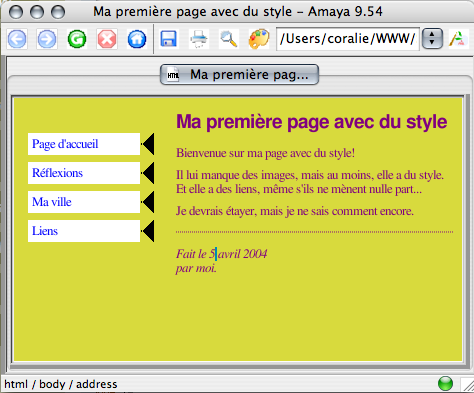
\includegraphics{voronin/img/capture5.png}
		\caption{Le texte principal a été déplacé à droite et la liste de liens est maintenant à sa gauche au lieu d'être au-dessus. }
		\label{fig:screen6}	
	\end{center}
\end{figure}
L'étape suivante est d'enregistrer les deux fichiers mapage.html et monstyle.css sur votre site Web. (Probablement après les avoir modifié un peu au préalable…) Mais cela dépend entièment de votre fournisseur d'accès Internet. 



\end{document}


\end{document}